% Chapter 1

\chapter{引言} % Main chapter title
\label{Chapter1} % For referencing the chapter elsewhere, use \ref{Chapter1} 
\section{背景介绍:从预测人口流动的城市危机防范到城市计算}
城市化进程催生了很多超大和大城市,并深远地改变了城市居民的生活状态和方式,然而,在带来众多生活上的便利的同时这也催生了诸如城市空气恶化、交通堵塞等重大挑战。在这其中,对于城市人口流动的管控和风险预测也显得十分重要。
预测城市人口的流动对于现代城市的安全和管理都是一个十分重要而充满挑战性的问题,而随着城市体量的增加和现代交通、信息等的发展,这一问题变得尤为重要。 2014年的新年夜,由于人流的急剧变化和缺乏应急预警,在上海外滩发生了造成36人死亡、47人受伤的惨痛踩踏事故\cite{hoang2016fccf:}。 试想,如果当时能有可以预测人流变化和区域流动的方法,对于这一区域进行及时的预警和疏导,就不会有这样的惨剧发生。\\
\indent 关于人流预测的先前研究集中于对于单个个体的活动的预测分析\cite{ye2009mining,zheng2012an}和对道路的交通状况的研究\cite{shang2014inferring,wang2014travel}。 尽管这些研究从一定程度上提供了对于城市的交通、人流的详细描述,但是由于整个城市的规模之大,要想对于整个城市或者城市的一部分进行这样的模拟来预测人口的流动在模拟能力和花费上是难以接受的;同时,对于整个城市的个体进行如此细致的模拟对于预测人口流动又显得没有必要。 另外,仅仅研究个体的行为无法揭示从群体层面上所会“涌现”出的诸多特征。这就使得研究者不得不思考运用新的研究方法和研究角度来分析和预测人口流动。\\
\indent 和传统的方法不同,由于现代的感知技术和大规模计算能力的成熟使得获取和计算和分析城市的巨量数据成为了可能,这也就催生出一个新的技术领域和框架——城市计算。这里将首先给出对于“城市计算”的基本介绍和核心要点以及其在预测城市人口流动这一问题中的结合和应用。\\
\indent 城市计算是一个获取、整合和分析城市空间中各种来源 (如传感器、设备、车辆、建筑物和人类) 生成的大型异构数据的过程, 并用以解决城市面临的主要问题\cite{zheng2014urban}。 城市计算连接无处不在的传感技术、先进的数据管理和分析模型以及新颖的可视化方法, 以改善城市环境、人类生活质量和城市运营体系。
\section{城市计算}
\subsection{框架}
如图\ref{fig:1.1}所示,城市计算主要由城市感知和数据获取、城市数据管理、城市数据分析和服务提供等环节构成。
\begin{figure}[ht]
\centering
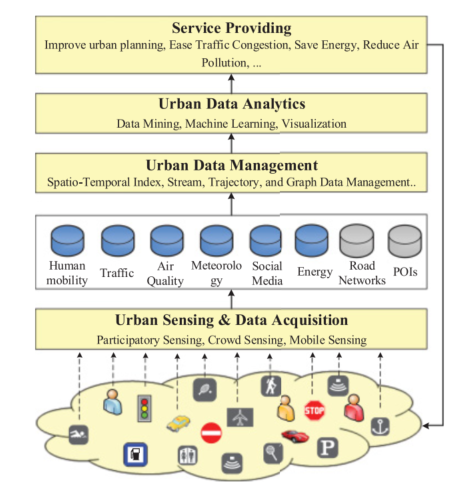
\includegraphics[width=0.8\textwidth]{frame.png}
\caption{城市计算的基本框架\cite{zheng2014urban}}
\label{fig:1.1}
\end{figure}
在城市感知阶段,主要利用固定的传感器和移动的如GPS信号、手机信号甚至社交媒体内容等多方面多维度的数据来源进行城市信息的收集;在城市数据管理阶段,将获得的不同来源甚至不同组织形式的数据进行结构化管理并进行和时间和空间上的对应以备后续分析;在数据分析环节,首先对于得到的组织数据进行模式分析,同时对于异常情况的发生可以进行准确的识别和预测;最后在服务提供阶段,对于异常的预测可以及时地对于相应的群体进行信息的分发还可以提供给城市的管理者进行及时的预警和调控。
\subsection{主要挑战}
和其他相对简单的系统相比,城市系统有着相对复杂的层级结构和纷繁的相互交织影响的动态信息,其作为一个动态复杂系统必然展现出诸如“涌现”等信息交织变化的特征\cite{anderson1972more},从而对于其的分析和预测必然面临着在不同层次和角度上的挑战。而城市计算主要有下面几个主要的挑战:
\subsubsection*{城市感知和数据获取}
在城市的大尺度下,想要连续地获得全面的数据显得十分困难。 例如,追踪某个区块的道路的车流相对可以实现,但是要连续追踪整个城市的车流由于传感器的分布和数据的传输等原因显得难以实现。 值得注意的是,相比传统的技术手段,在城市计算的框架下,人类所提供的信息或许可以成为这种传统的数据获取缺失的一种补充。 例如, 人在社交媒体上公开发表内容可能会提供周边环境的一些诸如交通、天气等的一些信息。 考虑到现代通讯的发达和城市人口的体量,这一信息来源蕴含着巨大的可以挖掘的信息,然而,这一新的数据来源再提供新的数据可能的同时也造成了新的问题:
\begin{itemize}
	\item 关于个人信息收集和隐私保护的问题
	\item 信息的难以控制和不均匀分布性。 传送信息的人的时间、地点、信息的内容、形式等式难以控制的,而且并不是能连续获得的,这也就造成了数据缺失和信息稀疏的问题,同时在城市中,无论从空间和时间上,从人类活动得到的信息都不是均匀分布的,这也对数据的分析造成了困难
	\item 由人所产生的数据可能是非结构化、不明显甚至充满噪声的,这和传统的传感器的信息可以直接用于清晰的解释和分析十分不同
\end{itemize}

\subsubsection*{异构数据的分析}
首先,城市计算所面临的数据往往是异构数据,也就是说对其进行分析和研究需要考虑一系列的复杂因素。 比如,对于空气质量的研究需要连续考量交通流、城市气象变化乃至土地区块利用情况等多重综合因素。 而现有的无论是数据挖掘还是机器学习等技术都只针对一种数据进行研究。 当然,一种简单的想法是将从不同的数据源提取的数据进行相同处理 (例如, 简单地
将这些特征放入要素向量并将其放入分类模型中),然而这种做法已经被证明预测的准确性相对较差\cite{yuan2012discovering}。 所以,如果采用多重的数据集进行分析会使得数据的维度增加,而这又加重了本就存在的数据集的稀疏问题, 如果这一问题没有被妥善处理,这甚至反而会造成模型的准确度下降。 \\
\indent 其次,城市计算的很多场景需要及时的预测和反馈,如空气污染、人流预测。这就要求分析手段既要保证分析的准确性还要保证其处理花费的有限性。
\\
\indent 最后,城市尺度的多维数据规模对于数据的可视化也提出了挑战,而数据分析结果的可视化能否提供足够清晰的信息也关系到其分析结果能否在灾害避免、交通疏导、空气治理等决策过程中发挥作用。

%\subsubsection*{虚拟世界和现实世界的交互}
%和传统的编写一个大型游戏或者是构建一个搜索引擎几乎完全在虚拟世界进行构建不同,城市计算从数据的获取、分析到最后的预测都不可避免的和城市的现实运行产生联系,这就给这样的系统的设计提出了新的信息交互和处理的挑战。

\subsection{城市信息}
之前提到,城市内部有着纷繁众多的信息来源,诸如地理信息、交通信息、手机信号、社交网络信息甚至经济运行的信息等多方面的信息。 在这一部分,本文将针对进行人流预测分析所主要依托的几个信息来源进行介绍和阐述。
\subsubsection*{地理信息}
地理信息主要包括路网信息和地理坐标信息,可以预料到,对于城市的诸多活动,路网都是一个很关键的因素,而位于其中的一些居住区、商场、餐厅的地理信息也对于分析十分重要。
\subsubsection*{交通信息}
交通的智能化和网联化,如打车服务软件的广泛使用使得对于一部分(出租车等)交通信息的实时收集变得可能,而城市道路上分布广泛的摄像头和传感器也提供了长期而巨量的交通监测信息。值得注意的是,广泛搭载GPS的车辆的运行可以提供连续的时空和轨迹信息。
\subsubsection*{移动手机}
由于移动手机实时和基站交换信息,通过这可以得到手机持有者的当前位置,再通过不同基站的信号可以获知其轨迹移动。由于智能手机的广泛使用,这一信息实际上提供了对于人流预测十分关键的基础信息。
\subsection{城市计算的技术手段}
为了应对之前所提到的三点挑战,研究者提出了很多技术和手段,其可以被大致分为以下四个方面:
\begin{itemize}
	\item 城市感知和数据处理技术
	\item 异构数据的融合技术
	\item 稀疏数据的处理方法
	\item 数据可视化的手段
\end{itemize}
\subsubsection*{城市感知和数据处理}
对于城市的数据获取,首先是依赖传统的传感器等手段进行数据的获取,其次可以通过对人群产生的数据进行处理得到所需求的数据,如可以通过网络信息的处理得到一些特定区块的餐饮经营状况。 \\
\indent 而对于数据的处理首先需要注意的是城市数据往往伴随着时间和空间信息,而处理机制需要能对于这样的复杂信息进行快速而有效的处理。现有研究中通常有三种结构来进行处理:流数据、轨迹数据和图数据。 在本文后面的人流预测的工作中将采取图数据的形式进行分析,这里一并对于其他两种处理形式进行简要介绍。
\subsubsection*{流数据和轨迹数据}
流数据在生活中十分常见,如温度数据、电的使用量和传感器的视频记录,都是时序的流数据,而对于流数据的研究和处理早已有了相对成熟的体系和方法\cite{Aggarwal2006Data},一系列成熟的DSMSs(Data stream management sysytems)系统(如 StreamInsight)等已经得到广泛应用。\\
\indent 而轨迹数据是指移动物体在地理空间移动形成的点的坐标连线,而诸如携带 GPS 的车辆和移动手机的信号都能生成轨迹数据。 而相比流数据而言,轨迹数据由于其和地理位置的高度相关和时序上的先后关联,传统的流数据的处理方法遇到了相当大的困难\cite{Wang2011Computing}。
\subsubsection*{图数据}
与流数据和轨迹数据不同,图数据是一种很好的表示交通系统,社交网络,人流分布的数据结构形式。 之前的研究主要集中对于静态的图数据的处理\cite{angles2008survey},而在城市计算中,往往是有一系列有着时序特征的图数据,也称为时空图\cite{hong2015detecting}(Spatiotemporal graph, ST graph),
而后序本文中所进行的预测分析的算法中就采用了这一数据形式对于人流进行预测分析。

\subsection{异构数据的融合技术}
在进行城市计算的过程中,需要利用很多的数据来源收集数据,这就必然要求要对不同来源和形式的数据进行统一化的处理从而进行下一步的分析。
现有的处理手段主要有以下三种:
\begin{enumerate}
	\item 在功能级别使用不同的数据源,即处理不同的数据源,同等地将从不同数据源提取的要素组合到一个特征向量。 需要注意的是,在分析前需要采用一定的方法对于数据进行归一化。这种方法也是目前采用最多的方法。
	\item 在不同的数据分析阶段采用不同的数据。 在文献中\cite{zheng2011urban}有将城市用路网划分为不同的区域再使用人的流动数据进行交通情况的预测分析。
	\item 将不同的数据输入到模型的不同部分。这一方法需要对于数据本身的深层理解才能构建出相对合理的模型,在实际的研究\cite{Zheng2013U,yuan2012discovering}中也发现基于对于数据的理解所构建的模型要显著好于前两种。
\end{enumerate}

\subsection{稀疏数据的处理方法}
尽管城市计算的数据规模非常之大,但是由于测量数据和测量手段的特点,依然会有数据缺失的问题,这就是是在计算机科学中经常需要处理的数据稀疏性的问题。 关于数据稀疏性的处理手段,常用和相对有效的有下面四种,在后文的工作中也会采取其中的方法对人口的信令数据进行预处理。
\subsubsection*{协作筛选}
协作筛选(Collaborative filtering, CF)被广泛使用在推荐系统的构建中,其基本的思想是相似的使用者对相似的物品有相似的评估标准和机制\cite{goldberg1992using}。 那么,如果可以确定出使用者和物品之间的联系,就可以对未来的使用者的评估做出预测\cite{nakamura1998collaborative}。 而在城市计算中, 物品可以是地理信息,乘客,司机还有服务的订购者。 一旦我们组装了矩阵,就可以使用这一准则来填充缺失的值。
\subsubsection*{矩阵分解}
矩阵分解,顾名思义就是讲矩阵分解为两个或者三个矩阵的乘积。 典型的方法有矩阵的 LU 分解、 QR 分解、 SVD 分解,其中 SVD 分解是使用最频繁的方法。 一种常用的方法为当矩阵非常稀疏时,可以使用三个低阶的矩阵对于其进行近似,比如只选取对应的奇异值之和大于总的奇异值之和的 \% 90 的那些行的数据。
\subsubsection*{张量分解}
张量通常有三个维度, 可以根据数据值对的特征分解为矩阵或向量的乘法。 限制分解的目标函数是最大限度地减少
中现有项的值的乘积。分解后, 我们通过
将分解后的矩阵或向量相乘可以填充张量中的缺失值。常常使用的主要有 PARAFAC\cite{bro1997parafac} 和 Tucker 分解\cite{kolda2009tensor}两种方法, 前者将张量分解为
三个向量的一系列乘积的总和, 而后者
用三个矩阵和一个核心张量的乘法近似一个张量。
\subsubsection*{半监督学习
}
半监督学习是一类监督学习任务和技术, 利用未标记的数据训练模型,其中通常包含少量标记的数据和大量未标记的数据。许多机器学习的研究人员发现, 未标记的数据, 当结合少量的标记数据,可以在学习精度方面有相当大的提高。 现有很多半监督的学习方法,如生成模型、基于图形的方法和协同训练。 具体来说,协同训练它假定每个实例都由两个
不同的功能集组成,这些功能集为每个实例提供了不同的和互补的信息。理想情况下, 每个实例的两个功能集都是有条件地独立,并且可以从每个视图准确地预测实例的分类。协同训练可以产生更好的推理结果, 因为其中一个分类器正确地标记了其他分类器以前错误分类的数据\cite{nigam2000analyzing}。\\

\subsection{数据可视化}
可视化以直观的方式帮助我们理解获取的知
识和模式。与单一数据可视化不同,城市计算中
的可视化技术需要同时考虑多个维度,其中,空间和时间是两个至关重要的维度\cite{zhengyu2015}。
\subsubsection*{降维和选取}
对于整体的数据进行可视化不失为一个好的方法,但是由于数据的高维性,选择对于数据进行一些降维处理再进行可视化,不失为一种很直观的展示手法。实际上,在后续的分析中,为了更好的揭示人口分布的规律,对于数据可视化的同时进行了聚类,使得更能展现出人口在空间上的分布特征。